\chapter{Basic Simplification Algorithm}
\thispagestyle{empty}% no page number in chapter title page
In this section I will present a basic algorithm for mesh simplification which is founded on serverl fundamental components: iterative vertex contraction, quadric error metric, mesh clustering and parallel strategy to consume those clusters. In this chapter I will elaborate each of those parts considering surface geometry alone. In the next chapter I will introduce the extended version of this algorithm which additionaly uses color and normals for the error metric.
\section{Design}
The core of the algorithm is based on Michael Garland's work Quadric-Based Polygonal Surface Simplification \cite{garland99} where he suggests an algorithm capable of producing high-quality approximations of polygonal meshes. The main assumption is that the approximation need not to maintain the topology of the original surface and is a nicely balanced trade of between quality and size. 

The goal of this work was to adopt this algorithm to a parallel framework capable of fast progresive mesh streaming [citation] for renderer engines in browsers. An example of such a renderer is Indoorviewer product created by NavVis. Depending on selected mesh resolution and level of details an appropriate mesh will be streamed to a browser. Therefore, the size and quality is crucial for the endpoint users to get maximal usability. Using the assumption that planar surfaces need much less trinagles to describe geometry we can get light and detailed meshes which are perfect for streaming purposes.

\section{Iterative Vertex Contraction}
The simplification algorithm is based on several atomic operations. One of them is an edge contraction. Let me denote an edge as a pair of vertices $(v_i, v_j)\longrightarrow\bar{v}$. The atomic opartion of a contraction is then defined as:

\begin{enumerate}
\item Move the vertices $v_i$ and $v_j$ to the position $\bar{v}$
\item Replace all connections of $v_j$ with $v_i$
\item Remove $v_j$ and all faces which belong both to $v_i$ and $v_j$. In Figure 2.1 the gray faces.
\end{enumerate}

\begin{figure}[h!]
  \begin{center}
        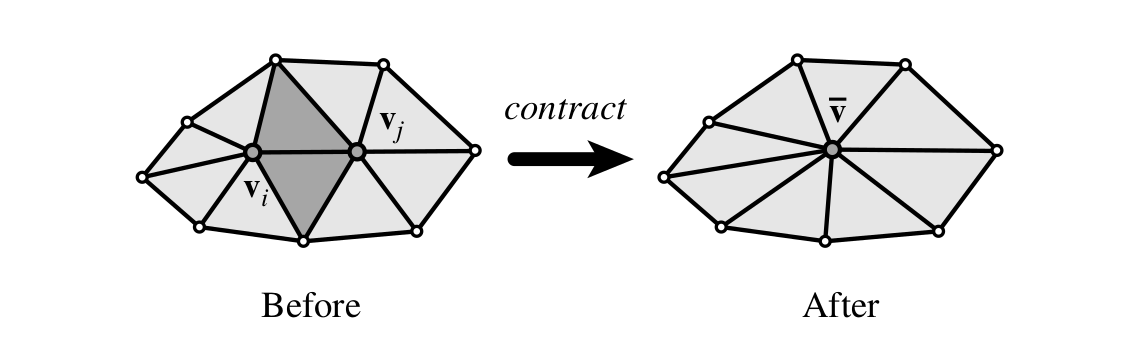
\includegraphics[width=17cm]{edge_contraction}
    \caption{Contraction of an edge}
    \label{fig:ToUseWithReference}
  \end{center}
\end{figure}

In the parallel framework the crucial aspect is locking all vertices and faces for the current edge to prevent from multiple threads modify the same region. To achieve this, $tryLock()$ method was used. To perform a contraction we have to check if it is possible to lock the whole neighbourhood, in the other case, it means that already a different thread is manipulating a given region. In such a situation the contraction is stopped.

The algorithm is a greedy procedure \cite{cormen01} driven by the cost of contraction. To achieve simplification we apply a sequence of edge contraction. Where the sequence is created as follows \cite{garland97}:

\begin{enumerate}
\item Select a set of candidate vertex pairs.
\item Assign a cost of contraction to each candidate.
\item Place all candidates in a heap keyed on cost with the minimum cost pair at the top.
\item Repeat until the desired approximation is reached:
\begin{enumerate}
\item Remove the pair $(v_i, v_j)$ of least cost from the heap.
\item Contract this pair.
\item Update costs of all candidate pairs involving $v_i$.
\end{enumerate}
\end{enumerate}

Each edge is associated with a cost of contraction which is basically the amount of error made during deletion of a given pair of vertices.  This cost is a key in the minimum heap \cite{cormen01} which is iteratively $pop()$. In each main iteration (steps from 1 to 4) we contract edges up to the current adaptive threshold level. If a current edge's cost is bigger or equal than the acceptable error, the main iteration procedure is stopped and the remaining egdes in the heap are ignored. In a next iteration the error is slightly increased in such a way that perviously contracted regions are even more simplified. The error calculations are based on a hyperparameter $aggressiveness$ and the current iteration value:
\[error(i)=0.000000001*(i+3)^a\]
where $i$ is the iteration and $a$ is the aggressiveness.
\section{Assessing Cost of Contraction}
Als Schrifttyp wird Arial oder Roman empfohlen. Bitte beachten, da�
Gr��en und Einheiten eine eigene Schreibweise haben:
\begin{description}
\item[Kursivschrift:] physikalische Gr��en (z.B.~$U$ f�r Spannung),
  Variablen~(z.B.~$x$), sowie Funktions- und Operatorzeichen, deren
  Bedeutung frei gew�hlt werden kann (z.B.~$f(x)$)
\item[Steilschrift:] Einheiten und ihre Vors�tze (z.B.~kg, pF),
  Zahlen, Funktions- und Operatorzeichen mit feststehender Bedeutung
  (z.B.~sin, lg)
\end{description} 

\clearpage

\chapter{Extended simplification algorithm}
\thispagestyle{empty}% no page number in chapter title page
\section{Design}
